\section{System Architecture} \label{sec:system_architecture}

% Provide a general view on main components and their tasks and interfaces; how is this system supposed to work; how do the components interact with each other
% Specify important definitions on components and data formally


\begin{figure}[b!]
    \centering
    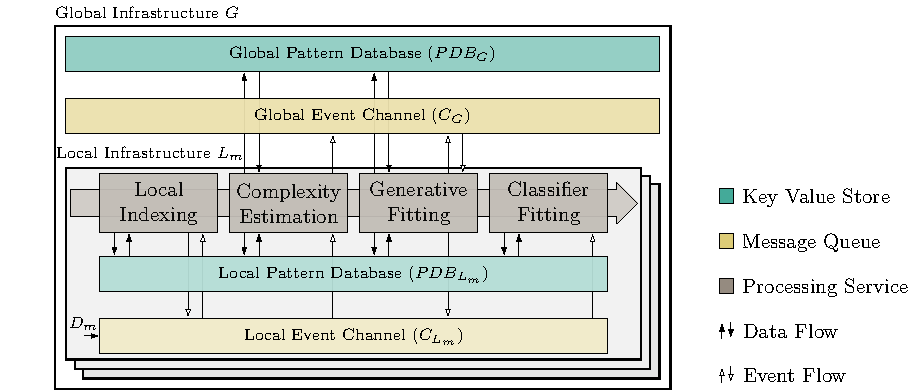
\includegraphics[width=1\linewidth]{tikz/detailed_architecture.pdf}
    \caption{High level CIDS architecture.}
    \label{fig:detailed_architecture}
    \end{figure}

    
    Logically, the proposed CIDS exhibits a hierarchical architecture (see Figure \ref{fig:high_level_architecture}). For one, the global infrastructure $G$ represents the collection of $M \in \mathbb{N}$ CIDS participants and their knowledge on an abstract level. For another, it provides specific services, that are globally available to each local infrastructure $L_m, m \in \{1, \dots, M\}$ that includes all CIDS components and processes within the IT infrastructure boundaries of a corresponding CIDS member. Each local infrastructure $L_m$ agrees to a specified feature extraction process that provides the monitoring data $\bm{X} \subset \mathbb{R}^d$ for the attack detection. Single data points of the monitoring data are referred to as $\bm{x} \in \bm{X}$ with a total number of features $d = |\bm{x}| \in \mathbb{N}$. In addition, the set of targets $Y \subset \mathbb{N}$ with instances $y \in Y$ is known and registered by every local infrastructure $L_m$. Furthermore, every $L_m$ prodives an individual training dataset $D_m= \{(\bm{x}_n, y_n): 1 \leq n \leq N_m\}$ of size $N_m = |D_m| \in \mathbb{N}$. CIDS communication across local boundaries occurs exclusively in a vertical direction. Thus, the exchange of information between individual $L_m$ takes place indirectly via the global pattern database $(PDB_G)$ and the global event channel $(C_G)$. Each $L_m$ includes a local pattern database $(PDB_{L_m})$, a local event channel $(C_{L_m})$ and an event-based data processing pipeline that consists of four services.

    \begin{table}[b]
        \centering
        
\begin{tabular}{ll} 
    \toprule
    \textbf{Notation} & \textbf{Description}             \\ 
    \midrule
    $G$                     & Global Infrastructure            \\
    $L_m$                   & Local Infrastructure $m$             \\
    \midrule
    $PDB_G, PDB_{L_m}$                   & Global Pattern Database, Local Pattern Database of $L_m$             \\
    $C_G, C_{L_m}$                     & Global Event Channel, Local Event Channel of $L_m$                    \\
    \midrule
    $M \in \mathbb{N}$      & Total number of CIDS participants         \\
    $m \in \{1, \dots, M\}  $         & Local Infrastructure Identifier  \\
    \bottomrule
\end{tabular}

        \caption{Summary of the architecture notation.}
    \end{table}

\subsection{Pattern Database} \label{subsec:pattern_database}

% what are the tasks of a pdb
depending on the scope (either local or global), different tasks are considered
local pdbs store intrusion detection datasets and corresponding metadata of the respective member; 
global pdbs store global metadata (combined information of local datasets) and the generative models


Each instance of a pattern database $(PDB)$ is realized as a key-value store. For the following algorithm descriptions, a $PDB$ is treated as a hash table as defined in Section \ref{subsec:hash_table}, that is referred to by replacing its function variable with the identifier of the corresponding database, e.g. $PDB_G(k)$ being a specific slot or hash value related to a key $k$ in the global pattern database. Note that if a specific hash function is already used to construct a key (e.g. Random Projection), the hash table will internally apply a distinct hash function on the key to ensure even distribution across the slots.

\subsection{Event Channel} \label{subsec:event_channel}
Event channels provide a topic-based publish-subscribe messaging mechanism that is mainly used to distribute workloads among the service instances in the processing pipeline. Via the messaging system, service instances receive and emit events, on which upon the respective operations are triggered. Changes in a pattern database result in responses that in turn are leveraged as the respective events. In this fashion, updates are propagated throughout the processing pipeline, ensuring a timely consistency among the pattern databases.

\subsection{Processing Pipeline} \label{subsec:processing_pipeline} 
Local and global pattern databases serve exclusively as data sources and sinks for operations. The only exception is the initial import of datasets $D_m$ into the \textit{Local Indexing} service via the messaging system.